\chapter{Arsitektur Continer (Container Architecture)}
\authors{Richwen Canady, Desfantio WUidjaja, Vincenzo Matalino}

\section{Latar Belakang}
Pada mulanya pengembangan perangkat lunak menyatukan fungsi-fungsi dari \textit{graphical user interface} (GUI) dan pengelolaan data ke dalam satu kode tanpa memisahkan mereka sesuai dengan perhatian (\textit{concerns}) mereka masing-masing. 
Konsekuensinya, pola tersebut akan menimbulkan masalah ketika \textit{developer} diminta untuk membangun aplikasi  skala besar,  misalnya aplikasi yang menolong pengguna berinteraksi dengan dataset yang besar dan kompleks. Kode program akan menjadi lebih tidak terstruktur (\textit{spaghetti code}) dan sulit untuk dipahami. 
Sebagai solusi, kode program perlu dibagi ke dalam komponen-komponen sesuai dengan perhatian mereka (\textit{separation of concerns}). 
Arsitektur Model-View-Controller (MVC) kemudian diajukan untuk membagi kode program ke dalam tiga abstraksi utama: \textit{model}, \textit{view}, dan \textit{controller}.
\subsection{Virtualization vs Container Architecture}

\section{Definisi Container dan Istilah-Istilah}
Container adalah pola arsitektur untuk pengembangan \textit{Graphical User Interface} (GUI). Arsitektur tersebut membagi logika progam menjadi 3 bagian yang saling terhubung: Model, View, dan Controller. Skema dari MVC dapat dilihat pada Gambar \ref{fig:mvc}..

\textbf{Docker} adalah 

\textbf{Kubernetes} merupakan presentasi yang ditampilkan ke pengguna yang dengannya pengguna dapat berinteraksi. Misalnya, halaman web, GUI desktop, diagram, \textit{text fields}, \textit{buttons}, dsb.

\textbf{Container Architecture} bertugas untuk

\begin{figure}[h]
    \centering
    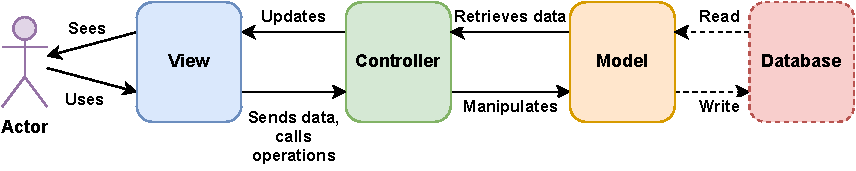
\includegraphics[width=\textwidth]{mvc}
    \caption{Arsitektur Container.}
    \label{fig:mvc}
\end{figure}

\section{Kelebihan dan Kekurangan}
Berikut adalah kelebihan dan kekurangan arsitektur MVC:


\subsection{Kelebihan}
Keuntungan dari menerapkan arsitektur MVC adalah:
\begin{itemize}
\item Pemisahan presentasi dan data membolehkan model ditampilkan di banyak \textit{view} secara bersamaan.
\item View bersifat \textit{composable} artinya view dapat dibangun dari berbagai atau berisi \textit{subviews}/\textit{fragments}.
\item Controller satu dapat diganti (\textit{switchable}) dengan controller lain pada saat \textit{runtime}.
\item Developer dapat membuat berbagai macam mekanisme pemrosesan data dari input ke output dengan mengkombinasikan berbagai macam fungsionalitas yang dimiliki oleh views, controllers, dan models.
\item \textit{Data engineers}, \textit{backend} dan \textit{frontend developers} masing-masing dapat fokus mengerjakan tugas utama mereka. 
Misal, \textit{data engineers} hanya mengerjakan tugas yang berkaitan dengan data, sendangkan \textit{frontend developers} fokus ke \textit{user interface}.
\end{itemize}

\subsection{Kekurangan}
Konsekuensi dari penerapan arsitektur MVC adalah sebagai berikut:
\begin{itemize}
\item Derajat kompleksitas kode program bertambah karena kode harus dibagi ke dalam tiga abstraksi yang berbeda.
\item \textit{Developers} harus mengikuti aturan ketat tertentu dalam mendefinisikan \textit{controllers}, \textit{models}, dan \textit{views}. 
\item Secara relative, MVC lebih sulit dipahami dikarenakan struktur bawaannya.
\item Terlalu berlebihan (\textit{overkill}) untuk aplikasi sederhana.
\item Cocok untuk pembangunan Graphical User Interface tetapi belum tentu cocok untuk pengembangan aplikasi atau komponen yang lain. 
\item Adanya lapisan-lapisan abstraksi dapat mengurangi kinerja (\textit{performance}) aplikasi.
\end{itemize}

\section{Contoh Kasus}

\subsection{Deskripsi}
Jelaskan contoh kasus yang dipaparkan berkaitan dengan arsitektur yang dimaksud pada bab ini.
Contoh kasus harus memperjelas arsitektur yang dimaksud.

\subsection{Penjelasan Implementasi}
Jelaskan bagian-bagian kode program, basisdata, atau konfigurasi yang signifikan terhadap arsitektur yang dimaksud.

\begin{lstlisting}[firstnumber=1,style=java,caption={Model dari \textsf{Rate}.},label=lst:rate_model]
import javax.persistence.Entity;
import javax.persistence.Id;
import javax.persistence.IdClass;

@Entity
@IdClass(RateId.class)
public class Rate {
  @Id
  private String fromCurrency;
  @Id
  private String toCurrency;
  private Double rate;
  ...
  Rate(String fromCurrency, String toCurrency, Double rate) {
    ...
  }
  ...
}
\end{lstlisting}

\begin{lstlisting}[firstnumber=1,style=java,caption={ \textsf{RateRepository}.},label=lst:rate_repository]
import java.util.Collection;
import org.springframework.data.jpa.repository.Query;
import org.springframework.data.repository.CrudRepository;

public interface RateRepository extends CrudRepository<Rate, Integer> {  
  @Query("SELECT r FROM Rate r WHERE r.fromCurrency = ?1 and r.toCurrency = ?2")
  Collection<Rate> findFirstByFromCurrencyAndToCurrency(String fromCurrency, String toCurrency);
  
  @Query("SELECT DISTINCT(r.fromCurrency) FROM Rate r")
  Collection<String> findAllFromCurrency();
  
  @Query("SELECT DISTINCT(r.toCurrency) FROM Rate r")
  Collection<String> findAllToCurrency(); 
}
\end{lstlisting}


\section{Kesimpulan}
Rangkum dan ulangi (beri penekanan pada) hal-hal kunci dari arsitektur yang dimaksud.


